\section{Preliminaries}


\subsection{BPaxos Graphs and Partial BPaxos Graphs}
\begin{floatingfigure}{0.3\textwidth}
  \centering
  \tikzstyle{vertex}=[]
  \tikzstyle{arrow}=[thick, -latex]

  \begin{subfigure}[b]{0.3\textwidth}
    \centering
    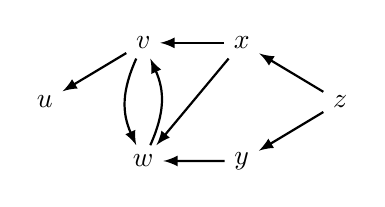
\begin{tikzpicture}[xscale=1.25, yscale=0.75]
      \node[vertex] (u) at (0, 0) {$u$};
      \node[vertex] (v) at (1, 1) {$v$};
      \node[vertex] (w) at (1, -1) {$w$};
      \node[vertex] (x) at (2, 1) {$x$};
      \node[vertex] (y) at (2, -1) {$y$};
      \node[vertex] (z) at (3, 0) {$z$};

      \draw[arrow] (v) to (u);
      \draw[arrow, bend right=15] (v) to (w);
      \draw[arrow, bend right=15] (w) to (v);
      \draw[arrow] (x) to (v);
      \draw[arrow] (x) to (w);
      \draw[arrow] (y) to (w);
      \draw[arrow] (z) to (x);
      \draw[arrow] (z) to (y);
    \end{tikzpicture}
    \caption{A conflict graph}\figlabel{ExamplePreCondensation}
  \end{subfigure}

  \begin{subfigure}[b]{0.3\textwidth}
    \centering
    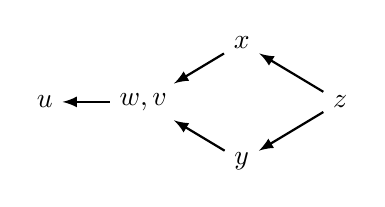
\begin{tikzpicture}[xscale=1.25, yscale=0.75]
      \node[vertex] (u) at (0, 0) {$u$};
      \node[vertex] (vw) at (1, 0) {$w,v$};
      \node[vertex] (x) at (2, 1) {$x$};
      \node[vertex] (y) at (2, -1) {$y$};
      \node[vertex] (z) at (3, 0) {$z$};

      \draw[arrow] (vw) to (u);
      \draw[arrow] (x) to (vw);
      \draw[arrow] (y) to (vw);
      \draw[arrow] (z) to (x);
      \draw[arrow] (z) to (y);
    \end{tikzpicture}
    \caption{The condensed conflict graph}\figlabel{ExampleCondensation}
  \end{subfigure}

  \caption{A conflict graph.}\figlabel{ExampleConflictGraph}
\end{floatingfigure}


Consider again a set $\Cmd$ of commands and a conflict relation $\conflict$. A
\defword{BPaxos graph} (with respect to $\Cmd$ and $\conflict$) is a directed
(potentially cyclic) graph $B = (V, E, \varphi)$ where
%
  $V$ is a set of vertices;
%
  $E \subseteq V \times V$ is a set of edges;
%
  $\varphi: V \to \Cmd$ is a function that labels every vertex with a command;
  and
%
  for every pair of vertices $v_1, v_2 \in V$, there exists an edge between
  $v_1$ and $v_2$ if (but not only if) $\varphi(v_1)$ and $\varphi(v_2)$
  conflict.
%
Intuitively, a BPaxos graph is a potentially cyclic conflict graph that can
have spurious edges between vertices labelled with non-conflicting commands.

A \defword{partial BPaxos graph} $B = (V, E, \varphi)$ is a BPaxos graph except
that $\varphi: V \partialto \Cmd$ is partial. Intuitively, a partial BPaxos
graph is a BPaxos graph for which the labels of some vertices are unknown.
%
We say a vertex $v$ in a partial BPaxos graph is \defword{eligible} if $v$ and
all vertices reachable from $v$ are labelled. The \defword{eligible suffix} of
a partial BPaxos graph $B$ is the suffix of $B$ consisting of all eligible
vertices.
%
An example partial BPaxos graph is illustrated in \figref{PartialBPaxosGraph},
and its eligible suffix is shown in \figref{EligibleSuffix}.

The \defword{condensation} of BPaxos graph $B$ is the graph obtained by first
removing spurious edges between non-conflicting vertices in $B$ and then by
contracting every strongly connected component. Every strongly connected
component labelled with commands $x_1, \ldots, x_n$ is replaced with a single
vertex labelled with a command string $x_{i_1} x_{i_2} \cdots x_{i_n}$ that is
obtained from an arbitrary but fixed ordering of the commands $x_1, \ldots,
x_n$. An example condensation is shown in \figref{Condensation}.
%
The condensation of a BPaxos graph with respect to $\Cmd$ and $\conflict$ is
a conflict graph with respect to $\Cmd^+$ and $\conflict^+$ where $\Cmd^+$ is
the set of non-empty command strings and where $(x_1 x_2 \cdots x_n, y_1 y_2
\cdots y_m) \in \conflict^+$ if there is some $x_i$ and $y_j$ that conflict in
$\conflict$.
